
% ----------------------------------------------------------------------
\section{Results}
\label{sec:results}
% ----------------------------------------------------------------------

\begin{figure}[t]
	\vspace*{2mm}
	\begin{center}
		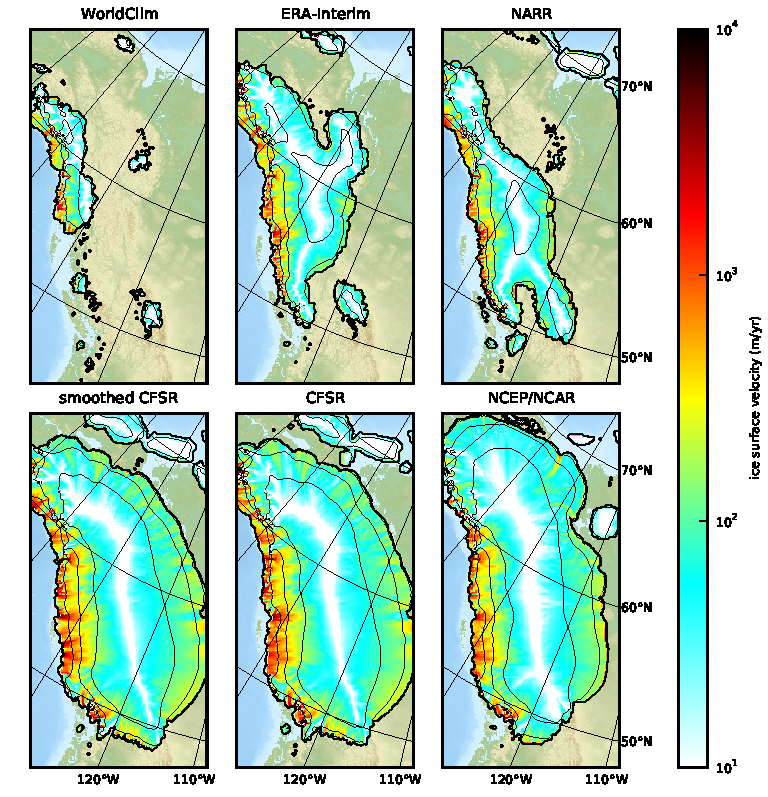
\includegraphics[width=13cm]{cordillera-climate-cool06}
	\end{center}
	\caption{Ice surface topography (black contours every 1000\,m) and velocity (\unit{m\,yr^{-1}}) after 10\,kyr under a climate 6\,\unit{\degree C} colder than present for each climate forcing.}
	\label{fig:cool06}
\end{figure}

\begin{figure}[t]
	\vspace*{2mm}
	\begin{center}
		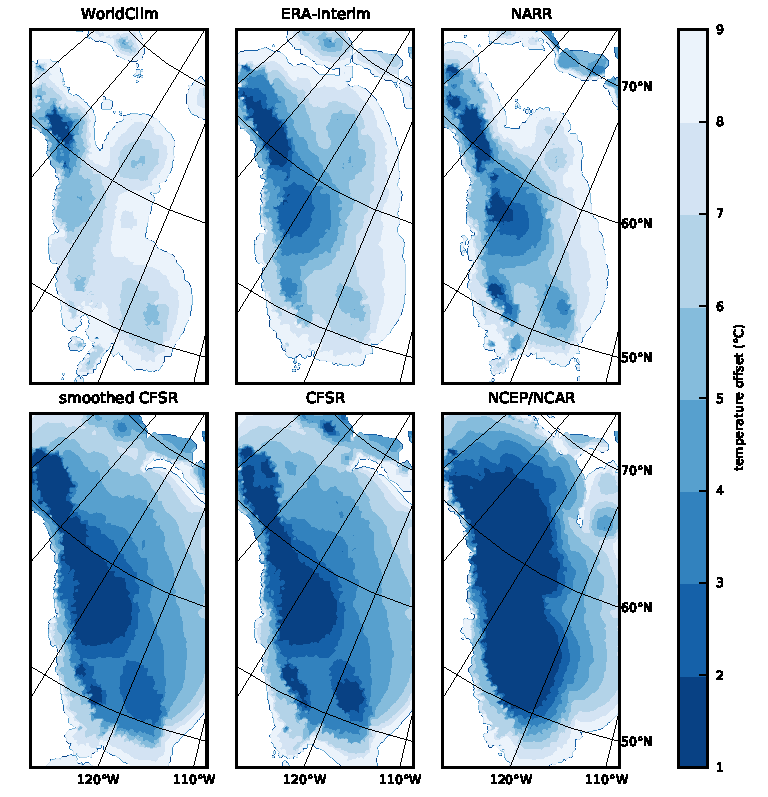
\includegraphics[width=13cm]{cordillera-climate-extent}
	\end{center}
	\caption{Extent of ice cover after 10\,kyr as a function of applied temperature offsets for each climate forcing.}
	\label{fig:extent}
\end{figure}

\begin{figure}[t]
	\vspace*{2mm}
	\begin{center}
		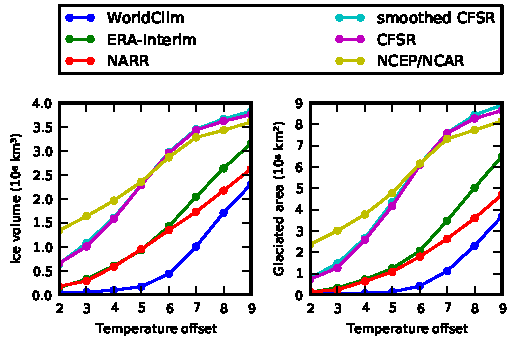
\includegraphics[width=9cm]{cordillera-climate-ivolarea}
	\end{center}
	\caption{Total ice volume and glaciated area after 10\,kyr as a function of temperature offset and climate forcing.}
	\label{fig:ivolarea}
\end{figure}

\begin{figure}[t]
	\vspace*{2mm}
	\begin{center}
		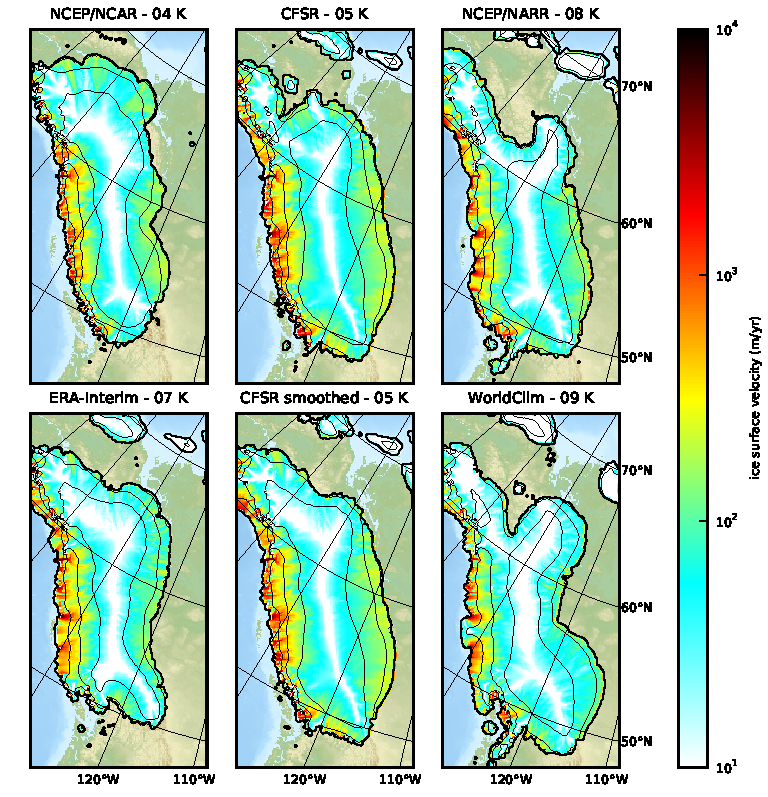
\includegraphics[width=13cm]{cordillera-climate-best}
	\end{center}
	\caption{Ice surface topography (black contours every 1000\,m) and velocity (\unit{m\,yr^{-1}}) after 10\,kyr using temperature offsets that lead to similar areas of ice cover for each climate forcing.}
	\label{fig:best}
\end{figure}

